\begin{ZhChapter}

\chapter{補充實驗}\label{chap:appendix}

除正文三個研究問題之三方法比較外，本研究另保留一項補充實驗以供參考：以 TAP-CT late fusion 進行之 GOLD 四分級分類。其樣本與早期訓練設定與主線 RQ 不完全一致，故不納入正文之三方法對齊比較，僅作為延伸觀察。

\section{GOLD 四分級分類}

GOLD 四分級依第三章 GOLD 2025 標籤設定，排除 Class 0（FEV1/FVC $\geq 70\%$，34 例），以 GOLD 1 至 GOLD 4 共 32 例（各類 2、11、13、6 例）進行四分類，並以 focal loss 訓練，結果如表~\ref{tab:rq5_gold_result} 與圖~\ref{fig:rq5_gold_cm} 所示。

\begin{table}[htbp]
\centering
\caption{補充實驗：GOLD 四分級分類結果（TAP-CT late fusion）}
\label{tab:rq5_gold_result}
\begingroup
\renewcommand{\arraystretch}{1.25}
\begin{tabular}{l c}
\hline
Metric & 5-fold average \\
\hline
Accuracy & $0.5429 \pm 0.0571$ \\
Macro-F1 & $0.3798 \pm 0.0870$ \\
Macro-Precision & $0.4042 \pm 0.0965$ \\
Macro-Recall & $0.4083 \pm 0.0553$ \\
Balanced Accuracy & $0.4083 \pm 0.0553$ \\
\hline
\end{tabular}
\endgroup
\end{table}

\begin{figure}[htbp]
\centering
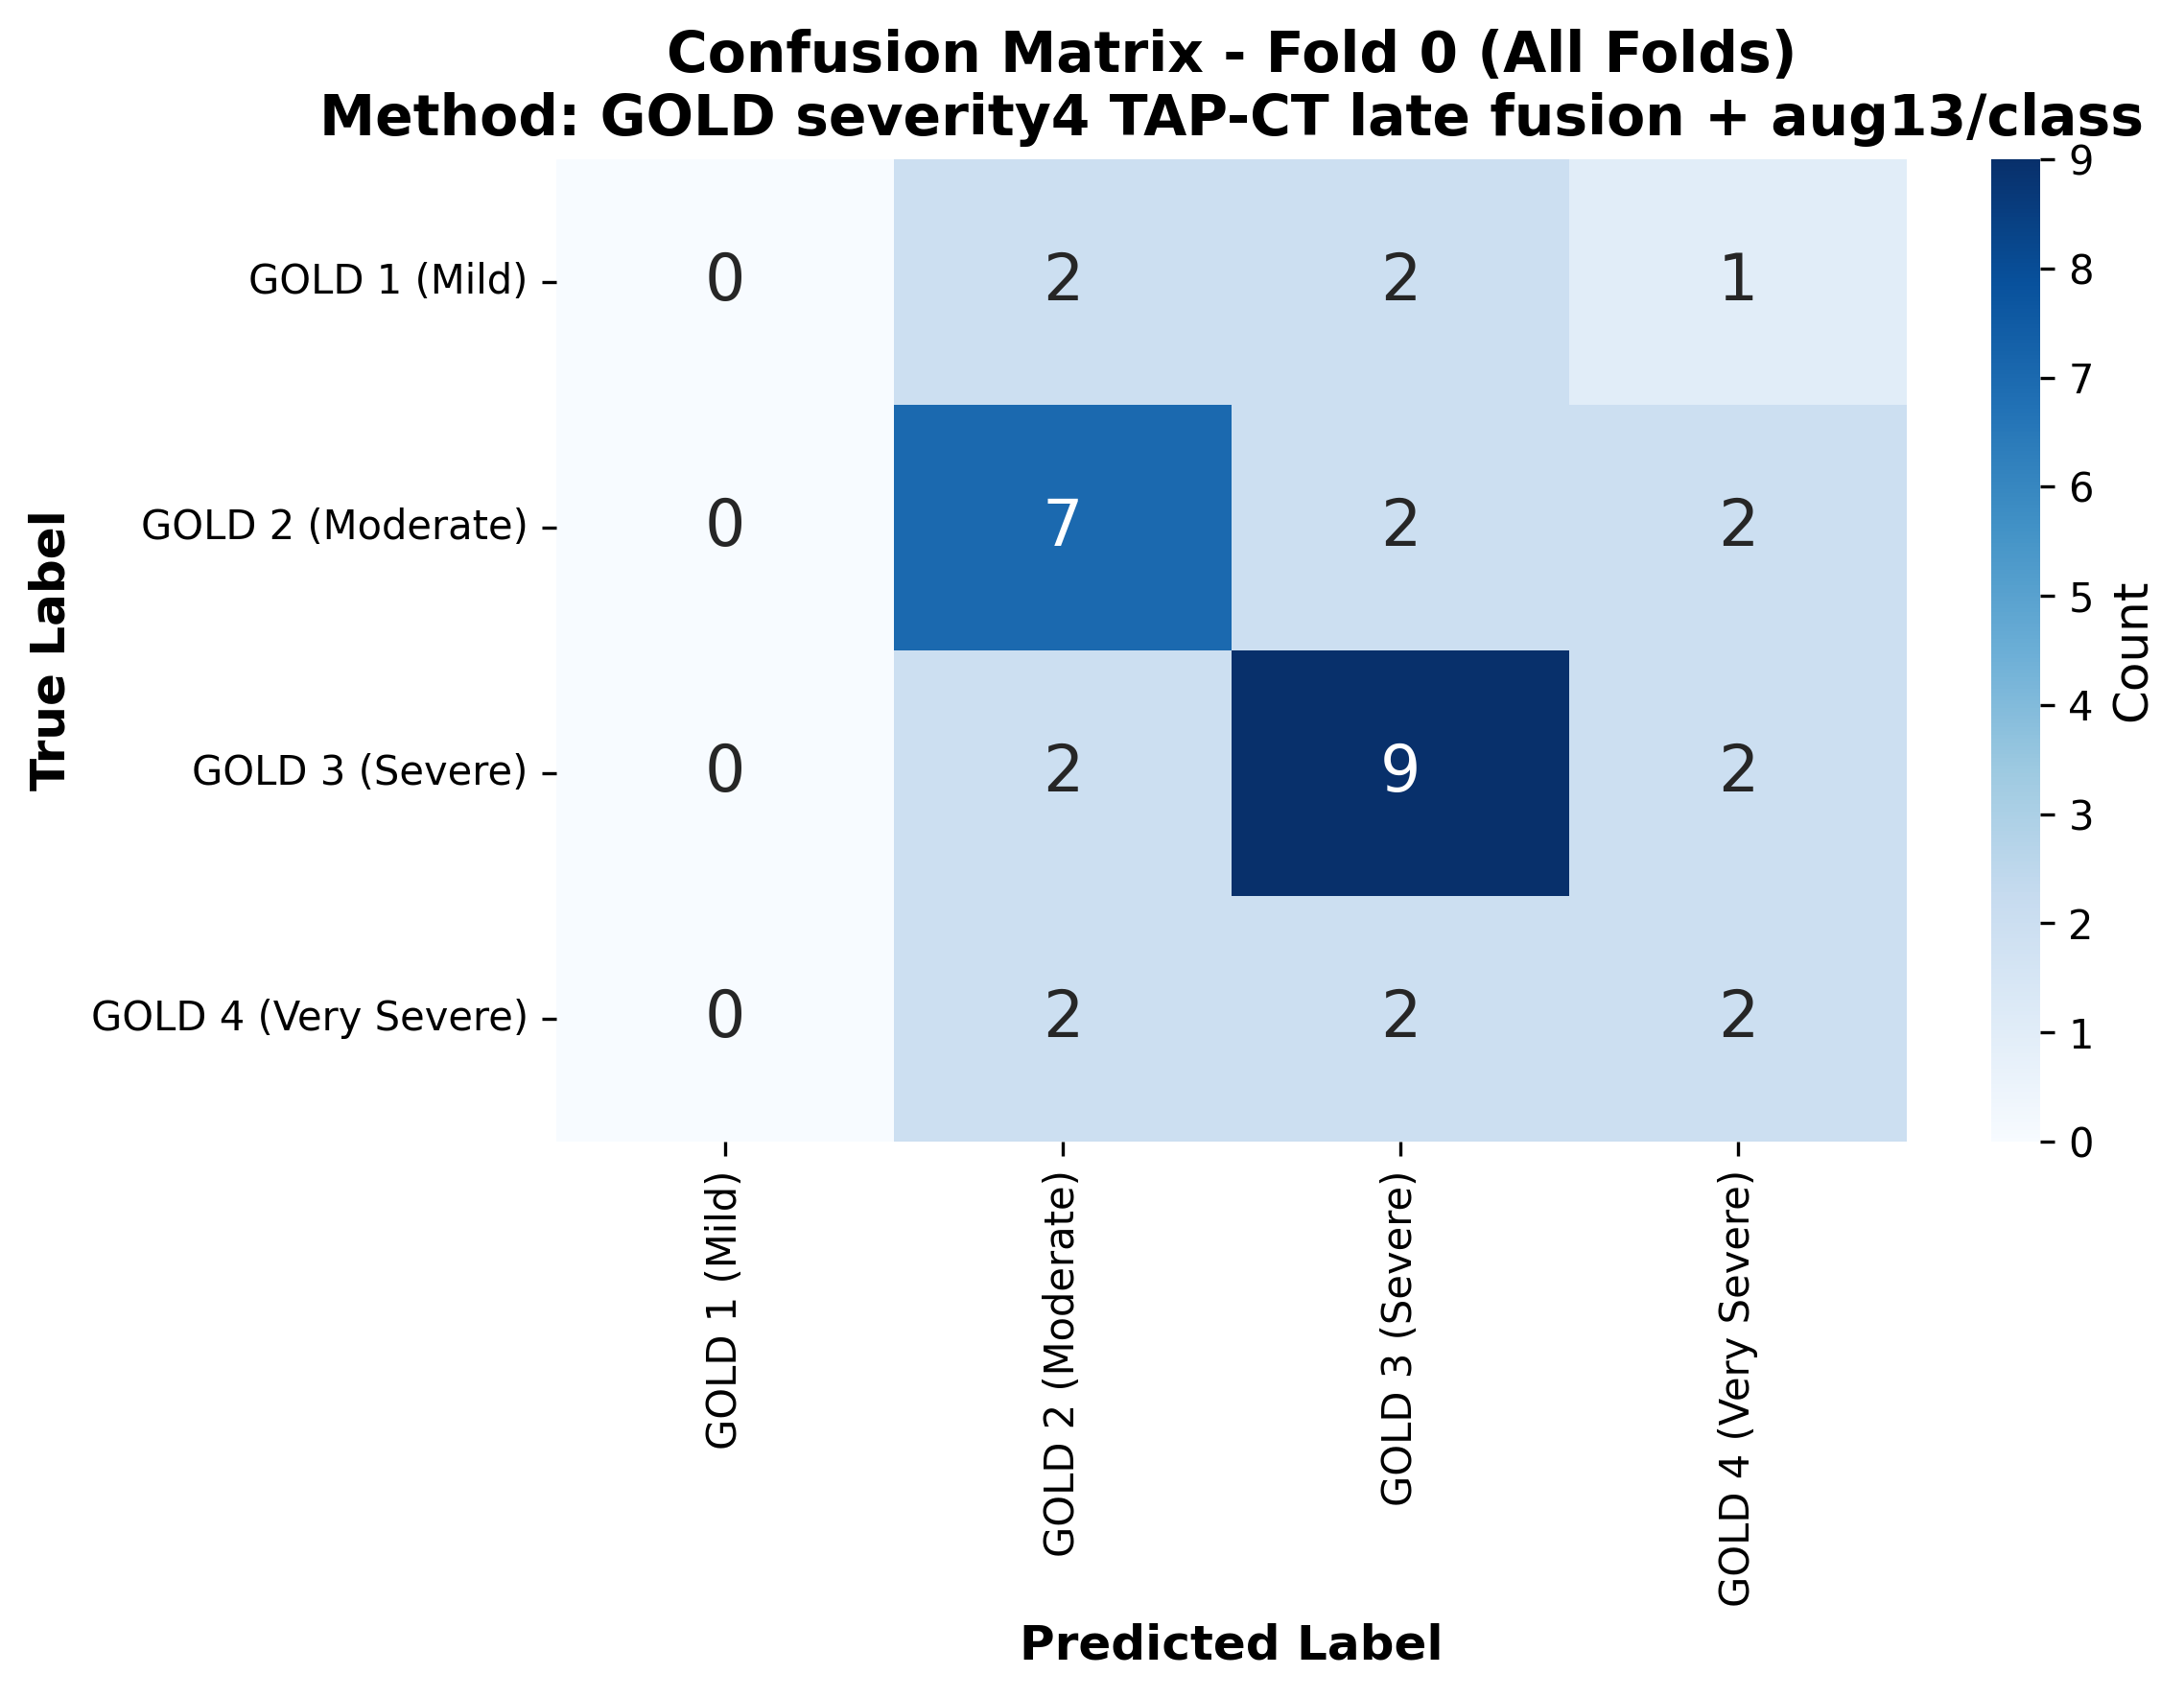
\includegraphics[width=0.82\textwidth]{figures/total_confusion_matrix.png}
\caption{補充實驗：GOLD 四分級分類混淆矩陣}
\label{fig:rq5_gold_cm}
\end{figure}

GOLD 四分級之五折平均 Accuracy 為 $0.5429 \pm 0.0571$、Macro-F1 為 $0.3798 \pm 0.0870$、Balanced Accuracy 為 $0.4083 \pm 0.0553$。由圖~\ref{fig:rq5_gold_cm} 可見，GOLD 3（13 例）與 GOLD 2（11 例）辨識相對較佳，GOLD 1（2 例）與 GOLD 4（6 例）兩端之極少樣本分級則為主要混淆來源；在 GOLD 1 樣本量極度不足之前提下，Balanced Accuracy 僅約 0.41，顯示資料不平衡是四分類可行性之主要限制。

\end{ZhChapter}
